\documentclass{beamer}

\usepackage[graphicx]
\usepackage{tikz-network}
\usepackage[table]{xcolor}

\title{Graph Theory}
\author{Melissa Carvajal, Carmen Hidalgo & Josu\'e Soto}
\institute{Investigaci\'on de Operaciones}
\date{2025}

\begin{document}
\maketitle

\begin{frame}
\frametitle{Floyd's Algorithm}
This program consists of Floyd's algorithm to obtain the shortest path between any pair of nodes in a graph with weighted distances.
Floyd's algorithm compares the distance between any two given nodes and by passing through another city in between, if the result is less than the original then it chooses the shortest one. After contemplating all nodes in the graph, the graph is guaranteed to have all the shortest distances between any two nodes in the graph. These changes are recorded in another matrix called P that helps determine the shortest path between any two nodes.
\end{frame}
\begin{frame}
\frametitle{Robert W. Floyd (1936–2001)}
\begin{figure}
\centering
\includegraphics[width=0.25	extwidth]{floyd.jpg}
\caption{\label{fig:floyd}Robert Floyd}
\end{figure}
Robert Willoughby Floyd was a computer scientist that lived from 1936 to 2001. He made great advances in computer science and developed an algorithm to find the shortest paths between any two nodes for a directed graph. He was awarded a Turing Award in 1978.
\end{frame}
\begin{frame}
\frametitle{Initial Graph}
\begin{center}
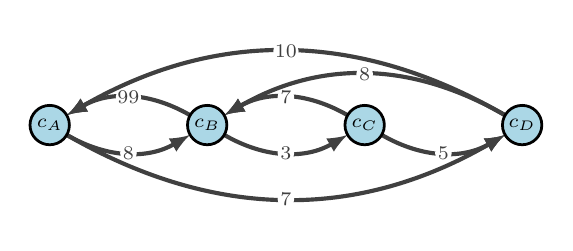
\begin{tikzpicture}
 \Vertex[x=0, y=0, size=0.5, label=$c_A$]{A}
 \Vertex[x=2, y=0, size=0.5, label=$c_B$]{B}
 \Vertex[x=4, y=0, size=0.5, label=$c_C$]{C}
 \Vertex[x=6, y=0, size=0.5, label=$c_D$]{D}
 
 \Edge[bend=-30, label=$8$, Direct](A)(B) 
 \Edge[bend=-30, label=$7$, Direct](A)(D) 
 \Edge[bend=-30, label=$99$, Direct](B)(A) 
 \Edge[bend=-30, label=$3$, Direct](B)(C) 
 \Edge[bend=-30, label=$7$, Direct](C)(B) 
 \Edge[bend=-30, label=$5$, Direct](C)(D) 
 \Edge[bend=-30, label=$10$, Direct](D)(A) 
 \Edge[bend=-30, label=$8$, Direct](D)(B)\end{tikzpicture}
\end{center}
\end{frame}



\begin{frame}
\frametitle{Table D$_{0}$}
\begin{center}
    \begin{tabular}{|c||c|c|c|c|}
        \hline
        \textbf{D} & \textbf{0} & \textbf{1} & \textbf{2} & \textbf{3} \\
        \hline
        \hline
        \textbf{0}& 0 & 8 & \infty & 7 \\
        \hline
        \textbf{1}& 99 & 0 & 3 & \infty \\
        \hline
        \textbf{2}& \infty & 7 & 0 & 5 \\
        \hline
        \textbf{3}& 10 & 8 & \infty & 0 \\
        \hline
    \end{tabular}
\end{center}


\end{frame}





\begin{frame}
\frametitle{Table P$_{0}$}
\begin{center}
    \begin{tabular}{|c||c|c|c|c|}
        \hline
        \textbf{P} & \textbf{0} & \textbf{1} & \textbf{2} & \textbf{3} \\
        \hline
        \hline
        \textbf{0}& 0 & 0 & 0 & 0 \\
        \hline
        \textbf{1}& 0 & 0 & 0 & 0 \\
        \hline
        \textbf{2}& 0 & 0 & 0 & 0 \\
        \hline
        \textbf{3}& 0 & 0 & 0 & 0 \\
        \hline
    \end{tabular}
\end{center}


\end{frame}





\begin{frame}
\frametitle{Table D$_{1}$}
\begin{center}
    \begin{tabular}{|c||c|c|c|c|}
        \hline
        \textbf{D} & \textbf{0} & \textbf{1} & \textbf{2} & \textbf{3} \\
        \hline
        \hline
        \textbf{0}& 0 & 8 & \infty & 7 \\
        \hline
        \textbf{1}& 99 & 0 & \cellcolor[HTML]{D74894}-2147483550 & \cellcolor[HTML]{D74894}106 \\
        \hline
        \textbf{2}& \infty & \cellcolor[HTML]{D74894}-2147483641 & 0 & \cellcolor[HTML]{D74894}-2147483642 \\
        \hline
        \textbf{3}& 10 & 8 & \cellcolor[HTML]{D74894}-2147483639 & 0 \\
        \hline
    \end{tabular}
\end{center}


\end{frame}





\begin{frame}
\frametitle{Table P$_{1}$}
\begin{center}
    \begin{tabular}{|c||c|c|c|c|}
        \hline
        \textbf{P} & \textbf{0} & \textbf{1} & \textbf{2} & \textbf{3} \\
        \hline
        \hline
        \textbf{0}& 0 & 0 & 0 & 0 \\
        \hline
        \textbf{1}& 0 & 0 & \cellcolor[HTML]{D74894}0 & \cellcolor[HTML]{D74894}0 \\
        \hline
        \textbf{2}& 0 & \cellcolor[HTML]{D74894}0 & 0 & \cellcolor[HTML]{D74894}0 \\
        \hline
        \textbf{3}& 0 & 0 & \cellcolor[HTML]{D74894}0 & 0 \\
        \hline
    \end{tabular}
\end{center}


\end{frame}





\begin{frame}
\frametitle{Table D$_{2}$}
\begin{center}
    \begin{tabular}{|c||c|c|c|c|}
        \hline
        \textbf{D} & \textbf{0} & \textbf{1} & \textbf{2} & \textbf{3} \\
        \hline
        \hline
        \textbf{0}& 0 & 8 & \cellcolor[HTML]{D74894}-2147483542 & 7 \\
        \hline
        \textbf{1}& 99 & 0 & -2147483550 & 106 \\
        \hline
        \textbf{2}& \cellcolor[HTML]{D74894}-2147483542 & -2147483641 & 0 & -2147483642 \\
        \hline
        \textbf{3}& 10 & 8 & -2147483639 & 0 \\
        \hline
    \end{tabular}
\end{center}


\end{frame}





\begin{frame}
\frametitle{Table P$_{2}$}
\begin{center}
    \begin{tabular}{|c||c|c|c|c|}
        \hline
        \textbf{P} & \textbf{0} & \textbf{1} & \textbf{2} & \textbf{3} \\
        \hline
        \hline
        \textbf{0}& 0 & 0 & \cellcolor[HTML]{D74894}1 & 0 \\
        \hline
        \textbf{1}& 0 & 0 & 0 & 0 \\
        \hline
        \textbf{2}& \cellcolor[HTML]{D74894}1 & 0 & 0 & 0 \\
        \hline
        \textbf{3}& 0 & 0 & 0 & 0 \\
        \hline
    \end{tabular}
\end{center}


\end{frame}





\begin{frame}
\frametitle{Table D$_{3}$}
\begin{center}
    \begin{tabular}{|c||c|c|c|c|}
        \hline
        \textbf{D} & \textbf{0} & \textbf{1} & \textbf{2} & \textbf{3} \\
        \hline
        \hline
        \textbf{0}& 0 & 8 & -2147483542 & 7 \\
        \hline
        \textbf{1}& 99 & 0 & -2147483550 & \cellcolor[HTML]{D74894}104 \\
        \hline
        \textbf{2}& -2147483542 & -2147483641 & 0 & -2147483642 \\
        \hline
        \textbf{3}& 10 & 8 & -2147483639 & 0 \\
        \hline
    \end{tabular}
\end{center}


\end{frame}





\begin{frame}
\frametitle{Table P$_{3}$}
\begin{center}
    \begin{tabular}{|c||c|c|c|c|}
        \hline
        \textbf{P} & \textbf{0} & \textbf{1} & \textbf{2} & \textbf{3} \\
        \hline
        \hline
        \textbf{0}& 0 & 0 & 1 & 0 \\
        \hline
        \textbf{1}& 0 & 0 & 0 & \cellcolor[HTML]{D74894}2 \\
        \hline
        \textbf{2}& 1 & 0 & 0 & 0 \\
        \hline
        \textbf{3}& 0 & 0 & 0 & 0 \\
        \hline
    \end{tabular}
\end{center}


\end{frame}





\begin{frame}
\frametitle{Table D$_{4}$}
\begin{center}
    \begin{tabular}{|c||c|c|c|c|}
        \hline
        \textbf{D} & \textbf{0} & \textbf{1} & \textbf{2} & \textbf{3} \\
        \hline
        \hline
        \textbf{0}& 0 & 8 & \cellcolor[HTML]{D74894}-2147483632 & 7 \\
        \hline
        \textbf{1}& 99 & 0 & -2147483550 & 104 \\
        \hline
        \textbf{2}& \cellcolor[HTML]{D74894}-2147483632 & -2147483641 & 0 & -2147483642 \\
        \hline
        \textbf{3}& 10 & 8 & -2147483639 & 0 \\
        \hline
    \end{tabular}
\end{center}


\end{frame}





\begin{frame}
\frametitle{Table P$_{4}$}
\begin{center}
    \begin{tabular}{|c||c|c|c|c|}
        \hline
        \textbf{P} & \textbf{0} & \textbf{1} & \textbf{2} & \textbf{3} \\
        \hline
        \hline
        \textbf{0}& 0 & 0 & \cellcolor[HTML]{D74894}3 & 0 \\
        \hline
        \textbf{1}& 0 & 0 & 0 & 2 \\
        \hline
        \textbf{2}& \cellcolor[HTML]{D74894}3 & 0 & 0 & 0 \\
        \hline
        \textbf{3}& 0 & 0 & 0 & 0 \\
        \hline
    \end{tabular}
\end{center}


\end{frame}


\begin{frame}
\frametitle{Final Graph}
\begin{center}
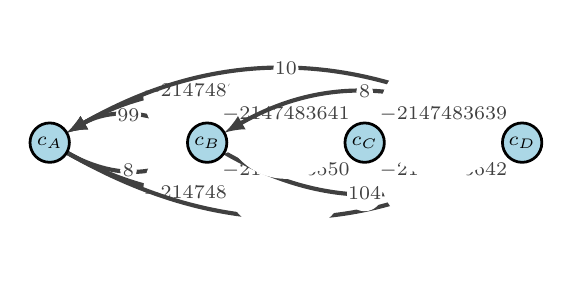
\begin{tikzpicture}
 \Vertex[x=0, y=0, size=0.5, label=$c_A$]{A}
 \Vertex[x=2, y=0, size=0.5, label=$c_B$]{B}
 \Vertex[x=4, y=0, size=0.5, label=$c_C$]{C}
 \Vertex[x=6, y=0, size=0.5, label=$c_D$]{D}
 
 \Edge[bend=-30, label=$8$, Direct](A)(B) 
 \Edge[bend=-30, label=$-2147483632$, Direct](A)(C) 
 \Edge[bend=-30, label=$7$, Direct](A)(D) 
 \Edge[bend=-30, label=$99$, Direct](B)(A) 
 \Edge[bend=-30, label=$-2147483550$, Direct](B)(C) 
 \Edge[bend=-30, label=$104$, Direct](B)(D) 
 \Edge[bend=-30, label=$-2147483632$, Direct](C)(A) 
 \Edge[bend=-30, label=$-2147483641$, Direct](C)(B) 
 \Edge[bend=-30, label=$-2147483642$, Direct](C)(D) 
 \Edge[bend=-30, label=$10$, Direct](D)(A) 
 \Edge[bend=-30, label=$8$, Direct](D)(B) 
 \Edge[bend=-30, label=$-2147483639$, Direct](D)(C)\end{tikzpicture}
\end{center}
\end{frame}
\end{document}
